\documentclass[]{VUMIFTemplateClass}

\usepackage{indentfirst}
\usepackage{amsmath, amsthm, amssymb, amsfonts}
\usepackage{mathtools}
\usepackage{physics}
\usepackage{graphicx}
\usepackage{verbatim}
\usepackage[hidelinks]{hyperref}
\usepackage{color,algorithm,algorithmic}
\usepackage[nottoc]{tocbibind}
\usepackage{tocloft}


\usepackage{titlesec}

\usepackage{biblatex}
\bibliography{bibliography}
%% norint pakeisti bibliografijos šaltinių numeravimą (skaitiniu arba raidiniu), pakeitimus atlikti VUMIFTemplateClass.cls 150 eilutėje

\usepackage{longtable}
\usepackage{booktabs}

\usepackage{gensymb}
\usepackage{acro}
\usepackage{tikz}
\usetikzlibrary{decorations.pathreplacing}
\usepackage{amssymb,amsthm}
\usepackage[version=4]{mhchem}
\usepackage{subcaption}

\input{setup/commands}
\studijuprograma{Programų sistemų} %Studijų programą įrašyti kilmininko linksniu (pavyzdžiui – Programų sistemų, Finansų ir draudimų matematikos ir t. t.)
\darbotipas{Bakalauro baigiamasis darbas} % Bakalauro baigiamasis darbas arba magistro baigiamasis darbas
\darbopavadinimas{Maišymo proceso modeliavimas YAG reakcijose}
\darbopavadinimasantras{Modelling the mixing process in YAG reactions}
\autorius{Arnas Vaicekauskas}

%Autorių gali būti ir daugiau, tuo atveju, kiekvienas autorius rašomas iš naujos eilutės, ir pridedamas titulinis.tex arba dvigubasTitulinis.tex dokumentuose
%\antrasautorius{Vardas Pavardė} %Jei toks yra, kitu atveju ištrinti

\vadovas{asist. dr. Rokas Astrauskas}
\recenzentas{prof. dr. (HP) Romas Baronas} %Jei toks yra žinomas, kitu atveju ištrinti
% \moksliniskonsultantas{pedagoginis/mokslinis vardas Vardas Pavardė} %Jei toks yra žinomas, kitu atveju ištrinti

\begin{document}

\selectlanguage{lithuanian}
\onehalfspacing
\input{titulinis}

%Turinys
\tableofcontents
\onehalfspacing

\sectionnonum{Įvadas}

Itrio aliuminio granatas (YAG) yra kristalinis junginys, pasižymintis išskirtinėmis optinėmis savybėmis. Dėl šių savybių YAG kristalai, legiruoti neodimio jonais, plačiai naudojami kaip lazerių aktyviosios terpės. Tokie lazeriai taikomi įvairiose srityse, įskaitant odontologiją \cite{valentiUseErYAG2021}, pramoninę gamybą \cite{dubeyExperimentalStudyNd2008} ir daugelį kitų.

YAG gali būti sintezuojamas keliais skirtingais būdais, įskaitant kietafazę reakciją, solvoterminį procesą, nusodinimą, purškiamojo aerozolio terminį skilimą ir zolio-gelio metodą. Daugelis šių metodų yra chemiškai sudėtingi ir reikalauja specializuotos laboratorinės įrangos. Tarp jų kietafazė reakcija išsiskiria kaip paprasčiausias ir pramoninei gamybai tinkamiausias sintezės būdas \cite{zhangNovelSynthesisYAG2005}. Šios reakcijos metu itrio ir aliuminio oksidai reaguoja aukštoje temperatūroje, susidarant YAG kristalams. Praktikoje reakcijos greitį galima padidinti periodiškai maišant reagentus. Maišymo momentas yra itin svarbus eksperimento vykdymo parametras, nes nuo jo priklauso bendra reakcijos trukmė. Šis ryšys tarp reakcijos trukmės ir maišymo laiko nėra iki galo ištirtas, todėl šiame tyrime jis bus analizuojamas taikant kompiuterinį modeliavimą.

Kompiuterinis fizinių bei cheminių procesų modeliavimas leidžia giliau suprasti ir tiksliau prognozuoti šių procesų eigą bei jų rezultatus. Šis tyrimo metodas taikomas daugybėje sričių, pavyzdžiui matematiniam biosensorių modeliavimui \cite{baronasNonlinearEffectsDiffusion2017, baronasNonlinearEffectsPartitioning2024}. Šis metodas itin naudingas analizuojant YAG sintezės reakciją, kadangi laboratoriniai eksperimentai suteikia ribotas galimybes detaliai ištirti vykstančius mechanizmus. Nors kompiuterinis modeliavimas taikomas jau ilgą laiką, jis išlieka aktualus ir šiandien. Matematinį YAG reakcijos modelį pasiūlė Ivanauskas ir bendraautoriai \cite{ivanauskasModellingSolidState2005}, o susijusiuose darbuose \cite{ivanauskasComputationalModellingYAG2009,mackeviciusCloserLookComputer2012} eksperimentiniu būdu buvo nustatytos fizinės modelio konstantos, todėl kompiuterinių skaičiavimų rezultatus galima lyginti su eksperimentiniais duomenimis. Minėtuose straipsniuose daugiausia dėmesio skirta pačios YAG sintezės reakcijos eigai ir koeficientų nustatymui, todėl reakcija buvo modeliuojama labai mažoje fizinėje srityje, kurioje telpa vos kelios mikrodalelės. Šiame darbe tiriamas maišymo mechanizmo poveikis reakcijai, kuris gali priklausyti nuo fizinės srities dydžio, todėl bus modeliuojamos įvairaus dydžio sritys siekiant įvertinti, ar maišymo modelių rezultatai yra patikimi.

Šią reakciją aprašo trijų netiesinių parabolinių dalinių diferencialinių lygčių sistema, sudaranti reakcijos-difuzijos modelį. Žinoma, kad tokiose netiesinėse sistemose analitinis sprendinys dažniausiai neegzistuoja, todėl jų sprendimui taikomi skaitiniai metodai. Vienas dažniausiai naudojamų metodų yra baigtinių elementų metodas (FEM), leidžiantis suskaidyti nagrinėjamą sritį į mažesnius elementus ir diferencialines lygtis spręsti kiekviename jų. Taip pat gali būti taikomas ribinių elementų metodas (BEM), kuris naudoja tik ribinių sąlygų informaciją ir yra ypač efektyvus sprendžiant uždavinius su sudėtingomis geometrijomis.

Šiame darbe reakcijos-difuzijos sistemai spręsti taikysime du baigtinių skirtumų metodus (FDM). Pirmasis — išreikštinis metodas, dar žinomas kaip Oilerio integracija. Šis metodas pasižymi paprastu įgyvendinimu, tačiau yra sąlyginai stabilus ir nėra itin tikslus. Antrasis — ADI (neišreikštinis kintamos krypties) metodas, kuris yra techniškai sudėtingesnis, tačiau nesąlyginai stabilus ir užtikrina didesnį skaičiavimų tikslumą \cite{doi:10.1137/0103003}. Be to, šis metodas leis efektyviai modeliuoti dideles erdvines sritis. Nors ADI metodas sukurtas jau seniai, jis vis dar plačiai taikomas įvairiuose skaitiniuose tyrimuose \cite{gaidamauskaiteComparisonFiniteDifference2007}. Abu šie skaitiniai metodai išsamiai aprašyti literatūroje \cite{pressNumericalRecipes3rd2007,levequeFiniteDifferenceMethods2007}.

Šio \textbf{darbo tikslas} — sudaryti skaitinius YAG reakcijos modelius ir, išanalizavus jų rezultatus, nustatyti, kokį poveikį maišymas daro reakcijos trukmei. Siekiant šio tikslo, buvo suformuluoti šie uždaviniai:

\begin{enumerate}
  \item Sudaryti kompiuterinius YAG reakcijos modelius, taikant išreikštinį ir ADI skaitinius metodus.
  \item Verifikuoti skaitinių modelių rezultatus, palyginti jų tikslumą ir efektyvumą.
  \item Apibrėžti medžiagų maišymo modelius.
  \item Integruoti medžiagų maišymo modelius į skaitinius YAG reakcijos modelius.
  \item Analizuoti skaitinių modelių rezultatus siekiant nustatyti, ar maišymo modelių savybės išlieka pastovios skirtingo dydžio srityse.
  \item Įvertinti, kaip reakcijos trukmė priklauso nuo maišymo momento, remiantis skaitinių modelių rezultatais.
\end{enumerate}

\input{sections/chemija}
% skyrius apie matematinį modelį

\section{Matematinis modelis}

Šiame darbe yra naudojamas (YAG) reakcijos modelis, kurį pasiūlė Ivanauskas et al \cite{ivanauskasModellingSolidState2005}. Reakcija yra modeliuojama kaip reakcijos-difuzijos sistema. Patį procesą modeliuosime dviejose dimensijose, stačiakampio srityje.

\begin{subequations} \label{rect}
	\begin{align}
		\frac{\partial c_1}{\partial t} & =-3kc_1c_2+D_1\left(\frac{\partial^2c_1}{\partial x^2}+\frac{\partial^2c_1}{\partial y^2}\right) \\
		\frac{\partial c_2}{\partial t} & =-5kc_1c_2+D_2\left(\frac{\partial^2c_2}{\partial x^2}+\frac{\partial^2c_2}{\partial y^2}\right) & (x, y, t)&\in\Omega\times[0, T]\\
		\frac{\partial c_3}{\partial t} & =2kc_1c_2+D_3\left(\frac{\partial^2c_3}{\partial x^2}+\frac{\partial^2c_3}{\partial y^2}\right)
	\end{align}
\end{subequations}

Čia $c_1,c_2,c_3$ yra medžiagų koncentracija, $t$ - laikas, $T$ - proceso trukmė, $W$ - stačiakampio plotis, $H$ - stačiakampio aukštis,
$D_i$ - atitinkamų medžiagų difuzijos konstantos, $k$ - reakcijos greičio konstanta, $\Omega=(0, W)\times(0, H)$ - stačiakampio sritis, kurioje vyksta reakcija. Srities $\Omega$ kraštinę žymėsime $\partial\Omega$:
\begin{align*}
    \partial\Omega=\{0, W\}\times[0, H]\cup[0, W]\times\{0, H\}
\end{align*}

Yra žinoma, kad reagentai difunduoja panašiu greičiu, todėl laikysime, kad $D_1=D_2$. Reakcijos produktas yra kristalas ir difunduoja daug lėčiau negu reagentai, todėl laikysime, kad $D_1 \gg D_3$.

Šios sistemos modelis yra uždaras - medžiagos neprateka pro stačiakampio srities kraštinę $\partial\Omega$, t.~y. taikoma Neumano kraštinė sąlyga:
\begin{align} \label{general-boundary-cond}
	\nabla c_m(x, y, t)\cdot\vec{n}&=0, & (x, y)&\in\partial\Omega & t&\in[0, T] & m&=1, 2, 3
\end{align}
Čia $\nabla c_m$ yra medžiagos $c_m$ gradientas, o $\vec{n}$ - paviršiaus $\partial\Omega$ normalė. Išskleidus kraštines sąlygas \eqref{general-boundary-cond} dviejose dimensijose gauname:
\begin{equation} \label{boundary-cond}
\begin{aligned}
\begin{split}
    \frac{\partial c_m}{\partial x}\Big|_{x=0}=\frac{\partial c_m}{\partial x}\Big|_{x=W}&=0 & y&\in[0,H] & t&\in[0, T] & m&=1, 2, 3\\
    \frac{\partial c_m}{\partial y}\Big|_{y=0}=\frac{\partial c_m}{\partial y}\Big|_{y=H}&=0 & x&\in[0,W] & t&\in[0, T] & m&=1, 2, 3
\end{split}
\end{aligned}
\end{equation}

\newpage
Ruošiant medžiagas reakcijai yra sudaromas stoichiometrinis medžiagų mišinys, todėl matematiniam modeliui yra taikomos šios pradinės sąlygos:
\begin{equation} \label{intial-cond}
	\begin{aligned}
		c_1(x, y, 0) & = \begin{cases} 3c_0, & \text{jei } (x, y)\in\Omega_1 \\ 0, & \text{kitaip} \end{cases} & \Omega_1&=\big(0, \tfrac{W}{2}\big]\times\big(0, \tfrac{H}{2}\big]\cup\big[\tfrac{W}{2}, W\big)\times\big[\tfrac{H}{2}, H\big)\\
		c_2(x, y, 0) & = \begin{cases} 5c_0, & \text{jei } (x, y)\in\Omega_2 \\ 0, & \text{kitaip} \end{cases} & \Omega_2&=\big(0, \tfrac{W}{2}\big)\times\big(\tfrac{H}{2}, H\big)\cup\big(\tfrac{W}{2}, W\big)\times\big(0, \tfrac{H}{2}\big)\\
		c_3(x, y, 0)&=0 & (x, y)&\in\overline{\Omega}=\Omega\cup\partial\Omega\\.
	\end{aligned}
\end{equation}

Čia $3c_0$ ir $5c_0$ atitinkamai yra medžiagų $c_1$ ir $c_2$ dalelių tankiai.

\begin{figure}[h!]
	\centering
	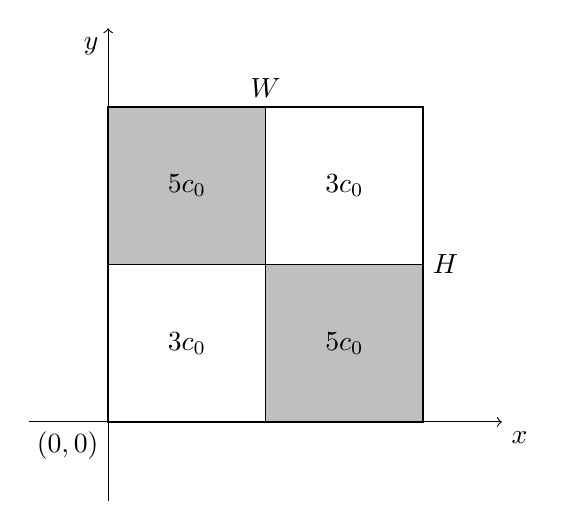
\begin{tikzpicture}[scale=2.0]
		\draw[fill=white] (0,0) rectangle (1,1);
		\draw[fill=white] (1,1) rectangle (2,2);
		\draw[fill=gray!50] (0,1) rectangle (1,2);
		\draw[fill=gray!50] (1,0) rectangle (2,1);

		% Draw the boundary of the square
		\draw[thick] (0,0) rectangle (2,2);

		% Draw axes
		\draw[->] (-0.5, 0) -- (2.5, 0) node[anchor=north west] {$x$};
		\draw[->] (0, -0.5) -- (0, 2.5) node[anchor=north east] {$y$};

		% Mark the origin
		\node[anchor=north east] at (0,0) {$(0, 0)$};

		% Mark the side length
		\draw[-] (2,0) -- (2,2) node[midway, right] {$H$};
		\draw[-] (0,2) -- (2,2) node[midway, above] {$W$};
		\draw (0.5, 1.5) node[anchor=center] {$5c_0$};
		\draw (1.5, 0.5) node[anchor=center] {$5c_0$};
		\draw (1.5, 1.5) node[anchor=center] {$3c_0$};
		\draw (0.5, 0.5) node[anchor=center] {$3c_0$};
	\end{tikzpicture}
	\caption{Sistemos pradinės sąlygos srityje $\Omega$. Tamsesnė spalva žymį sritį $\Omega_2$, o šviesesnė $\Omega_1$}
	\label{fig:initial-condition-visual}
\end{figure}
\section{Skaitiniai modeliai}

\subsection{Erdvės diskretizavimas}

Abiems skaitiniams modeliams naudosime tokiu pačiu principu sukonstruotą tinklelį. Jį sudarydami padaliname stačiakampę erdvę $\Omega$ į $N\times M$ taškų, kurie yra nutolę vienas nuo kito fiksuotais atstumais $\Delta x$ ir $\Delta y$ atitinkamomis ašimis. Analogiškai, laiko erdvę $[0, T]$ padalinsime į $\tau + 1$ taškų, kurie vienas nuo kito yra nutolę tolygiais $\Delta t$ atstumais. Apibūdinta diskretų tinklelį galima užrašyti taip:

\begin{align}
    \omega_W&=\{ x_i : x_i = i\Delta x, \quad i=0, 1, \dots, N - 1 \} & \Delta x&=\frac{W}{N-1} \label{meshx}\\
    \omega_H&=\{ y_j : y_j = j\Delta y, \quad j=0, 1, \dots, M - 1 \} & \Delta y&=\frac{H}{M-1} \label{meshy}\\
    \omega_\tau&=\{ t_n : t_n = n\Delta t,\quad n=0, 1, \dots, \tau\} & \Delta t&=\frac{T}{\tau} \label{mesht}\\
	\omega&=\omega_W\times\omega_H\times\omega_\tau \label{mesh}
\end{align}

\begin{figure}[!h]
\centering
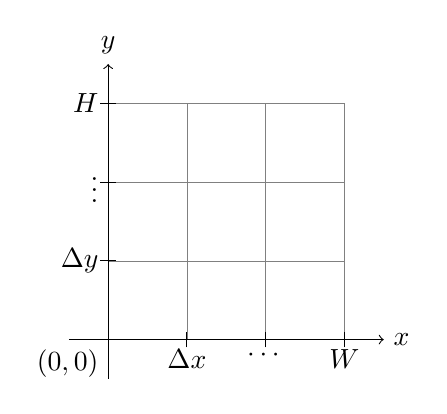
\begin{tikzpicture}
    
% Define the size of the cells
\def\Deltax{1} % Delta x size
\def\Deltay{1} % Delta y size
\def\Xmax{4} % Max X value
\def\Ymax{4} % Max Y value

% Draw the mesh
\foreach \x in {0,1,2} {
    \foreach \y in {0,1,2} {
        \draw[help lines] (\x*\Deltax,\y*\Deltay) grid (\x*\Deltax+\Deltax,\y*\Deltay+\Deltay);
    }
}

\node[below left] at (0,0) {$(0, 0)$};

% Draw axes
\draw[->] (-0.5,0) -- (3.5 *\Deltax,0) node[right] {$x$} ;
\draw[->] (0,-0.5) -- (0,3.5) node[above] {$y$};

% Add tick marks on x-axis with labels
\draw[shift={(1,0)}] (0,-0.1) -- (0,0.1);
\node[below] at (1, 0) {\(\Delta x\)};

\draw[shift={(2,0)}] (0,-0.1) -- (0,0.1);
\node[below] at (2, 0) {$\cdots$};

\draw[shift={(3,0)}] (0,-0.1) -- (0,0.1);
\node[below] at (3, 0) {$W$};

% Add tick marks on y-axis with labels

\draw[shift={(0,1)}] (-0.1,0) -- (0.1,0);
\node[left] at (0, 1) {$\Delta y$};
        
\draw[shift={(0,2)}] (-0.1,0) -- (0.1,0);
\node[left] at (0, 2) {$\vdots$};

\draw[shift={(0,3)}] (-0.1,0) -- (0.1,0);
\node[left] at (0, 3) {$H$};

\end{tikzpicture}
\caption{ Diskretizuota erdvė }
\end{figure}

\newpage

\subsection{Išreikštinis FTCS metodas}

Remiantis išreikštiniu FTCS (\textit{angl. forward time centered space}) metodu pakeisime sistemos \eqref{rect} lygtis su išvestinių aproksimacijomis gautomis skleidžiant išvestines pagal Teiloro eilutę.

\begin{subequations} \label{finite-diffs}
\begin{align}
	\frac{\partial c}{\partial t}\Big|_{x=x_i, y=y_j, t=t_n}&=\frac{c^{n+1}_{i,j}-c^n_{i,j}}{\Delta t} + \mathcal{O}(\Delta t)\\
    \frac{\partial^2c}{\partial x^2}\Big|_{x=x_i, y=y_j, t=t_n}&=\frac{c^n_{i-1,j} - 2c^n_{i,j} + c^n_{i+1,j}}{(\Delta x)^2} + \mathcal{O}((\Delta x)^2)\\
    \frac{\partial^2c}{\partial y^2}\Big|_{x=x_i, y=y_j, t=t_n}&=\frac{c^n_{i,j-1} - 2c^n_{i,j} + c^n_{i,j+1}}{(\Delta y)^2} + \mathcal{O}((\Delta y)^2)
\end{align}
\end{subequations}

Įstate aproksimacijų išraiškas gauname dvimatį skaitini modelį:

\begin{subequations} \label{numerical-eqs}
	\begin{align}
		\frac{c^{n+1}_{1,i,j}-c^n_{1,i,j}}{\Delta t} & =
		-3kc^{n}_{1,i,j}c^{n}_{2,i,j}\notag\\
        & +D\left(\frac{c^n_{1,i-1,j}-2c^n_{1,i,j}+c^n_{1,i+1,j}}{(\Delta x)^2}+\frac{c^n_{1,i,j-1}-2c^n_{1,i,j}+c^n_{1,i,j+1}}{(\Delta y)^2}\right) \\
		\frac{c^{n+1}_{2,i,j}-c^n_{2,i,j}}{\Delta t} & =
		-5kc^{n}_{1,i,j}c^{n}_{2,i,j}\notag\\
        &+D\left(\frac{c^n_{2,i-1,j}-2c^n_{2,i,j}+c^n_{2,i+1,j}}{(\Delta x)^2}+\frac{c^n_{2,i,j-1}-2c^n_{2,i,j}+c^n_{2,i,j+1}}{(\Delta y)^2}\right) \\
		\frac{c^{n+1}_{3,i,j}-c^n_{3,i,j}}{\Delta t} & =2kc^{n}_{1,i,j}c^{n}_{2,i,j},
	\end{align}
\end{subequations}

Čia
$\Delta t$ - laiko žingsnis,
$\Delta x$ - diskrečios erdvės žingsnis $x$ ašimi,
$\Delta y$ - diskrečios erdvės žingsnis $y$ ašimi.
$c^n_{1,i,j}$, $c^n_{2,i,j}$, $c^n_{3,i,j}$ - atitinkamai pirmos, antros ir trečios medžiagų koncentracijos diskretizuotos erdvės tinklelio taške $(x_i, y_i, t_n)\in\omega$.

\subsection{Neišreikštinis kintamos krypties metodas}

% Ka galima butu rasyti apie sita metoda
% kontekstas, is kur jis, kam skiras, pliusai ir minusai

Neišreikštinį kintamos krypties metodą (\textit{alternating direction implicit, ADI}) JAV mokslininkai Donald W. Peaceman ir Henry H. Rachford Jr. pristatė savo straipsnyje \enquote{skaitinis sprendinys parabolinėms ir elipsinės diferencialinėms lygtims}. Nuo to laiko šis metodas plačiai taikomas matematinio modeliavimo srityje. Kaip galima suprasti iš straipsnio pavadinimo, šis metodas pritaikytas spręsti parabolines ir elipsines diferencialinių lygčių sistemas, ypatingai tada, kai sistema turi daugiau nei vieną erdvinę dimensiją. Kadangi mūsų nagrinėjamą sistemą sudaro parabolinės diferencialinės lygtys jį ir taikysime.

Šis metodas yra tarpinis variantas tarp Išreikštinio FTCS ir Crank-Nicholson metodo, kuriuo bandoma išlaikyti sprendimo greitį, tačiau taip pat ir tikslumą. Įprastoms parabolinėms lygtims šis metodas būna besąlygiškai stabilus \cite{liAlternatingDirectionImplicit2021}, tai leidžia pasirinkti bet kokio dydžio laiko žingsnį ir tokiu būdu sumažinti bendrą laiko žingsnių kiekį, kurį reikia įvykdyti. Toliau pritaikysime metodą nagrinėjamai sistemai.

Tarkime turime skaitinį sprendinį konkrečių laiko momentu $t^n$, kaip ir anksčiau, jį žymėsime $c^n$. Vietoje to, kad tiesiogiai skaičiuotume skaitinį sprendinį sekančiu laiko momentu $c^{n + 1}$, apskaičiuosime tarpinį sprendinį, kurį žymėsime $c^*$. Šis sprendinys ypatingas tuo, kad jo ieškodami $x$ dimensiją laikysime išreikštine, o $y$ dimensiją -- neišreikštine:

\begin{align}
    \frac{c^* - c^n}{\frac{1}{2}\Delta t} = ...
\end{align}


\input{sections/skaitinis-stabilumas}
\input{sections/palyginimas}

\section{Maišymo modeliavimas}

\subsection{Atsitiktinis maišymas}

Konstruojant kompiuterinį modelį šiam procesui atkreipsime dėmesį į kelias svarbias detales:

\begin{itemize}
  \item Išmaišymas vyksta prie daug žemesnės temperatūros negu reakcija
  \item Išmaišymas gali vykti kelis kartus
  \item Išmaišymo procesas nėra deterministinis
\end{itemize}

\subsubsection*{Maišymas prie žemesnės temperatūros}

Kadangi maišymas vyksta prie daug žemesnės temperatūros negu pati reakcija, darysime prielaidą, kad ištraukus reagentus iš krosnies cheminė reakcija ir difuzija nevyksta, todėl medžiagų maišymą modeliuosime kaip momentinį procesą, kuris įvyksta tarp diskrečių laiko žingsnių.

\subsubsection*{Maišymas kelis kartus}

Praktikoje vykdant šią reakcija chemikai savo nuožiūra pasirenka laiką, kuriuo vykdys išmaišymą, todėl ir kompiuterinis modelis turėtų suteikti vartotojui pasirinkimą nurodyti konkrečius laiko momentus, kada vyks medžiagų išmaišymas. Šiuos laikus žymėsime taip:

\begin{align}
    t^1_\text{mix}, t^2_\text{mix}, \dots, t^{T^*}_\text{mix} \quad T^*\in \mathbb{N}
\end{align}

Čia $T^*$ -- bendras išmaišymų skaičius, o $t^i_\text{mix}$ -- $i$-tojo išmaišymo laikas. Kadangi kompiuterinis modelis laiko informaciją apie diskrečius laiko taškus $t_n$, mes negalime tiesiogiai apibrėžti sąlygos, kad išmaišymas vyks konkrečiu laiko momentu $t^i_\text{mix}$, todėl medžiagas išmaišysime einamajame laiko žingsnyje $t_n$, kuris yra artimiausias išmaišymo laikui $t^i_\text{mix}$:

\begin{figure}[!h]
\centering
\label{mix-inequality-graphic}
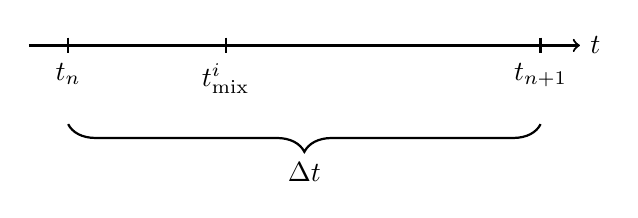
\begin{tikzpicture}[thick]

% Main timeline
\draw[->] (-0.5,0) -- (6.5,0) node[right] {$t$}; % Timeline with axis label

% Time points
\foreach \x/\label in {0/{$t_n$}, 2/{$t^i_\text{mix}$}, 6/{$t_{n+1}$}} {
    \draw (\x,0.1) -- (\x,-0.1) node[below] {\label};
}

% Braces for interval
\draw[decorate,decoration={brace,amplitude=10pt,mirror}] (0,-1) -- (6,-1) node[midway,below=10pt] {$\Delta t$};


\end{tikzpicture}
\caption{Šiuo atveju, išmaišymas įvyks laiko žingsniu $t_n$, o ne $t_{n+1}$, nes $t^i_\text{mix}$ yra arčiau laiko momento $t_n$}
\end{figure}

arba kitaip sakant išmaišymas įvyks laiko žingsniu $t_n$, jei:

\begin{align}
    \vert t_n - t^i_\text{mix} \vert < \frac{1}{2}\Delta t \label{mix-inequality}
\end{align}

\newpage

\subsubsection*{Atsitiktinis maišymas}

Maišymas praktikoje yra chaotiškas procesas, todėl sudarydami kompiuterinį modelį turime į tai atsižvelgti. Maišymą modeliuosime kaip reakcijos erdvės sričių atsitiktinį išdėstymą. Pradinė sritį $\Omega$ padalinsime į mažesnes, nepersidengiančias, vienodas kvadratines sritis $\Omega_i$, tada sugeneruosime atsitiktinę $4$-permutaciją $\sigma$ ir $4$ atsitiktinius kampus $\theta_i \in \{0, \frac{\pi}{2}, \pi, \frac{3\pi}{2}\}$. Kiekviena iš sričių $\Omega_i$ keliauja į poziciją, kurioje yra sritis $\Omega_{\sigma(i)}$, tačiau pasukta kampu $\theta_i$. 

\begin{figure}[!h]
\centering
\label{split-reaction-space}

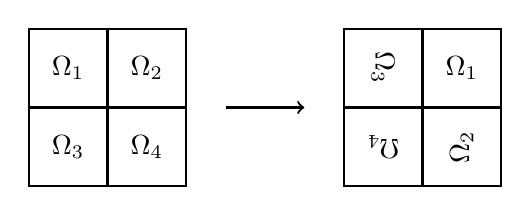
\begin{tikzpicture}
    % Original Grid
    \draw[thick] (0,0) rectangle (2,2);
    \draw[thick] (1,0) -- (1,2);
    \draw[thick] (0,1) -- (2,1);

    \node at (0.5,1.5) {$\Omega_1$};
    \node at (1.5,1.5) {$\Omega_2$};
    \node at (0.5,0.5) {$\Omega_3$};
    \node at (1.5,0.5) {$\Omega_4$};

    % Arrow
    \draw[->, thick] (2.5,1) -- (3.5,1);

    % Transformed Grid
    \begin{scope}[shift={(4,0)}]
        \draw[thick] (0,0) rectangle (2,2);
        \draw[thick] (1,0) -- (1,2);
        \draw[thick] (0,1) -- (2,1);

        \node at (0.5,1.5) {\rotatebox{270}{$\Omega_3$}}; % Rotated 180° horizontally
        \node at (1.5,1.5) {$\Omega_1$};             % No change
        \node at (0.5,0.5) {\rotatebox{180}{$\Omega_4$}}; % Upside down
        \node at (1.5,0.5) {\rotatebox{90}{$\Omega_2$}};  % 90° rotation
    \end{scope}
\end{tikzpicture}
\caption{Maišymo transformacijos pavyzdys}
\end{figure}

\begin{figure}[h]
    \centering
    \begin{minipage}[c]{0.40\textwidth}
        \centering
        \includegraphics[width=\textwidth]{images/rnd-mix-left-c0-1.png}\\
        \includegraphics[width=\textwidth]{images/rnd-mix-left-c1-1.png}\\
        \includegraphics[width=\textwidth]{images/rnd-mix-left-c2-1.png}
    \end{minipage}%
    \hfill
    \begin{minipage}[c]{0.1\textwidth}
        \centering
        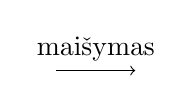
\begin{tikzpicture}
            \draw[->] (0,0.5) -- (1,0.5);
            \node[above] at (0.5, 0.5) {maišymas};
        \end{tikzpicture}
    \end{minipage}%
    \hfill
    \begin{minipage}[c]{0.45\textwidth}
        \centering
        \includegraphics[width=\textwidth]{images/rnd-mix-right-c0-1.png}\\
        \includegraphics[width=\textwidth]{images/rnd-mix-right-c1-1.png}\\
        \includegraphics[width=\textwidth]{images/rnd-mix-right-c2-1.png}
    \end{minipage}

    \caption{Atsitiktinis maišymo modelis pritaikytas skaitiniame modelyje. Maišymo laikas $t^1_\text{mix} = 1\text{h}\,30\text{min}$ }

    \label{fig:random-mix-example}

\end{figure}

\ref{fig:random-mix-example}-ame pavyzdyje matome kaip atrodo reakcijos eiga, kada vyksta išmaišymas. Trečiame stulpelyje ir ypatingai trečios medžiagos koncentracijoje matome ryškių artefaktų. Taip yra todėl, kad nuo išmaišymo praejo labai mažai laiko ir medžiagos nespėjo sureaguoti naujoje aplinkoje. Tarp laiko momentų $t=1h\,30min$ ir $t=5h\,59min$ trečios medžiagos $c_3$ koncentracija daugiausiai keitėsi tose vietose, kuriose iš pradžių vyko reakcija, tačiau galime matyti ir visiškai naujos sienelės susidaryma ties srities viduriu. Norint geriau suprasti kokį poveikį toks išmaišymas turi reakcijos pabaigos lakui reikėtų ištirti trečios medžiagos koncentracijos priklausomybę nuo laiko.

\newpage
\begin{figure}[h!]
    \centering
    \includegraphics[width=0.45\textwidth]{images/bad-mix-qnt-1.png}
    \caption{Kompiuterinio modelio rezultatų palyginimas, kai išmaišymas vyksta ir nevyksta.  }
    \label{bad-mix-qnt-example}
\end{figure}
\ref{bad-mix-qnt-example}-ame pavyzdyje puikiai matosi, kad išmaišymas nepagreitino reakcijos, o ją sulėtino. Reakcijos laikas su išmaišymu yra apytiksliai dvejom su puse valandom ilgesnis. Ši problema atsiranda todėl, kad mes modeliuojame ypač mažą reakcijos erdvės sritį, kurioje susiduria tik 4 mikrodalelės, dėl to nėra daug skirtingų išdėstymų, kada viena sienele galėtų dalintis skirtingų medžiagų dalelės, prie to žinoma prisideda ir faktas, kad šis modelis yra dviejų dimensijų. Eksperimentas parodė, kad nesuveiktų ir statistinis bandymas - vidutinis atsitiktinis išmaišymas taip pat neduoda geresnių rezultatų negu reakcijos modelis be išmaišymų. Dėl šios priežasties apsvarstysime alternatyvų išmaišymo metoda.

\subsection{Tobulas maišymas}

Kad išspręstume atsitiktinio maišymo problemą, modeliuosime tobulą teorinį išmaišymą, kuris turės didžiausią poveikį reakcijos greičiui. Pats maišymo modelis išliks toks pat, tačiau sritis $\Omega_i$ sudėliosime ne atsitiktinai, o sukeisime įstrižai. Tobulas išmaišymas aišku priklauso nuo pradinių sąlygų, o šis galioja tik duotoms pradinėms sąlygoms \eqref{intial-cond}.

\begin{figure}[!h]
\centering
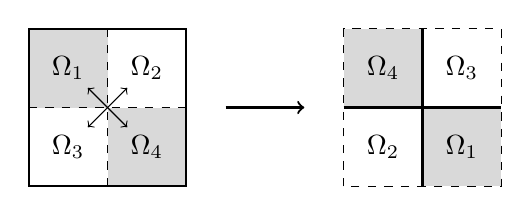
\begin{tikzpicture}
    % Original Grid
    \fill[gray!30] (0,1) rectangle (1, 2);
    \fill[gray!30] (1,0) rectangle (2, 1);
    \draw[<->] (0.75,0.75) -- (1.25,1.25);
    \draw[<->] (1.25,0.75) -- (0.75,1.25);
    \draw[thick] (0,0) rectangle (2,2);
    \draw[dashed] (1,0) -- (1,2);
    \draw[dashed] (0,1) -- (2,1);

    \node at (0.5,1.5) {$\Omega_1$};
    \node at (1.5,1.5) {$\Omega_2$};
    \node at (0.5,0.5) {$\Omega_3$};
    \node at (1.5,0.5) {$\Omega_4$};

    % Arrow
    \draw[->, thick] (2.5,1) -- (3.5,1);

    % Transformed Grid
    \begin{scope}[shift={(4,0)}]
        \fill[gray!30] (0,1) rectangle (1, 2);
        \fill[gray!30] (1,0) rectangle (2, 1);
        
        \draw[dashed] (0,0) rectangle (2,2);
        \draw[thick] (1,0) -- (1,2);
        \draw[thick] (0,1) -- (2,1);

        \node at (0.5,1.5) {$\Omega_4$};
        \node at (1.5,1.5) {$\Omega_3$};
        \node at (0.5,0.5) {$\Omega_2$};
        \node at (1.5,0.5) {$\Omega_1$};
    \end{scope}
\end{tikzpicture}
\caption{Tobulo maišymo transformacija}
\label{perfect-2x2-mix}
\end{figure}
\ref{perfect-2x2-mix}-ame pavyzdyje matoma prieš tai apibūdintą transformacija. Punktyrinės linijos kairėje pusėje žymi sieneles ties kuriomis vyksta reakcija. Šiuo atveju po išmaišymo nėra sričių, kurios turėtų bendrą punktyrinę sienelę, o tai reiškia, kad tokiu būdu sumaišius sritis, visos vidinės sienelės turės didžiausią įmanomą skirtingų medžiagų kontrastą, kuris lems didžiausią įmanomą reakcijos pagreitėjimą.

\subsubsection*{Tobulo maišymo rezultatai}

\begin{figure}[h!]
  \centering
  \includegraphics[width=0.75\textwidth]{images/mixing/perfect-mix-ord-0-c1.png} \\ 
  \includegraphics[width=0.75\textwidth]{images/mixing/perfect-mix-ord-0-c3.png}
  \caption{Tobulo maišymo poveikis skaitiniame sprendinyje. Modelio parametrai atitinka reakciją vykstančia $1000\degree C$ temperatūroje. Modeliuojamos srities rezoliucija $40\times40$. Išmaišymo laikas -- $1\text{h}. $}
  \label{fig:perfect-mix-small-example}
\end{figure}

\ref{fig:perfect-mix-small-example}-ame pavyzdyje matome kaip tobulas maišymo procesas paveikia reakcijos erdvę. Kaip ir su atsitiktinio maišymo modelio atveju, kokybiniai maišymo modelio rezultatai nėra pastebimi iš tokio reakcijos erdvės vaizdavimo, todėl analizuosime medžiagos kiekio priklausomybę nuo laiko.

\newpage

\begin{figure}[h!]
    \centering
    \includegraphics[width=0.5\textwidth]{../paper/images/mixing/perfect-mix-vs-no-mix-ord-0-q3.png}

    \caption{Kompiuterinio modelio rezultatų palyginimas tarp reakcijos be išmaišymo ir reakcijos su tobulu išmaišymu.  }

    \label{optimal-mix-qnt}
\end{figure}

Šiuo atveju, \ref{optimal-mix-qnt}-ame pavyzdyje matome, kad dėl tobulo išmaišymo galime matyti šuolį medžiagos kiekyje. Toks maišymas turi teigiamą poveikį reakcijos pabaigos laikui ir labiau atitinka eksperimentinius rezultatus negu atsitiktinis išmaišymas.
Čia galime pasamprotauti, kaip reakcijos pabaigos laikas priklauso nuo išmaišymo laiko - jei išmaišome pradinę konfigūraciją pačioje reakcijos pradžioje, rezultatams tai neturės jokios įtakos ir gausime reakcijos modelį be išmaišymo. Lygiai tas pats nutiktų jei išmaišymas įvyktų ką tik prieš reakcijos pabaigą, tačiau išmaišymas kitais laiko momentais, kaip jau matėme, gali sutrumpinti reakcijos pabaigos laiką. Jei pavaizduotume reakcijos trukmės priklausomybę nuo išmaišymo momento, gautume štai tokį grafiką:

\begin{figure}[h!]
    \centering
    \includegraphics[width=0.5\textwidth]{../paper/images/mixing/duration-mix-moment-dependance-ord0.png}

    \caption{Reakcijos trukmės priklausomybė nuo išmaišymo momento. Modelio parametrai atitinka reakciją $1000\degree C$ temperatūroje. Modeliuojamos srities rezoliucija $40\times40$. }

    \label{fig:duration-mix-moment-graph-for-small-space}
\end{figure}

\ref{fig:duration-mix-moment-graph-for-small-space}-ame pavyzdyje matome, kad priklausomybė nėra simetriška, reakcijos pabaigos laikas, kai išmaišymas nevyksta, yra apie 12val. Optimalus išmaišymo laikas yra apie 40min ir tokiu atveju 97\% medžiagų sureaguos per 11h 7min.

\newpage

\subsection{Reakcijos modeliavimas didesnėje srityje}

Modeliuoti mažą visos reakcijos erdvės sritį užtenka norint gauti tikslias aproksimacijas difuzijos bei reakcijos greičio konstantoms \cite{mackeviciusCloserLookComputer2012}. Tačiau modeliuodami medžiagų išmaišymą neturime priežasties daryti tokios pačios prielaidos. Norint modeliuoti didesnę erdvės sritį, pradines sąlygas reikia atkartoti veidrodiniu principu, tuo galima įsitikinti pažvelgus į \ref{fig:periodic-space}-ą pavyzdį. Modeliuojant didesnę erdvę, ne tik padidės srities plotas, kaip pavaizduota \ref{large-initial-conditions}-ame pavyzdyje, tačiau ir padvigubinsime diskrečių taškų kiekį kiekviena erdvine kryptimi. Šį procesą galima rekursyviai kartoti ir tokiu būdu gauti eksponentiškai didesnės srities pradines sąlygas.


\begin{figure}[h!]
\centering
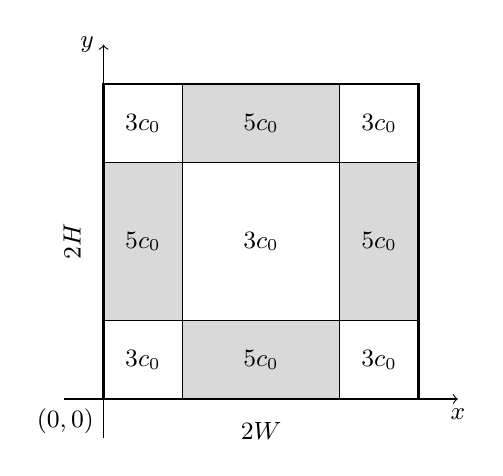
\begin{tikzpicture}
  
    % Fill the boundary cells
    % \fill[gray!30] (0, 3) rectangle (1, 4); % Top-left
    \fill[gray!30] (1, 3) rectangle (3, 4); % Top
    % \fill[gray!30] (3, 3) rectangle (4, 4); % Top-right
    \fill[gray!30] (0, 1) rectangle (1, 3); % Left
    \fill[gray!30] (3, 1) rectangle (4, 3); % Right
    % \fill[gray!30] (0, 0) rectangle (1, 1); % Bottom-left
    \fill[gray!30] (1, 0) rectangle (3, 1); % Bottom
    % \fill[gray!30] (3, 0) rectangle (4, 1); % Bottom-right

    % Draw the outer rectangle
    \draw[thick] (0, 0) rectangle (4, 4);
    \node at (2, -0.4) {\small $2W$};
    \node[rotate=90] at (-0.4, 2) {\small $2H$};

    % Draw the inner rectangle
    \draw[-] (0, 1) -- (4, 1);
    \draw[-] (0, 3) -- (4, 3);
    \draw[-] (1, 0) -- (1, 4);
    \draw[-] (3, 0) -- (3, 4);

    % Labels
    \node at (0.5, 3.5) {\small $3c_0$};
    \node at (2, 3.5) {\small $5c_0$};
    \node at (3.5, 3.5) {\small $3c_0$};

    \node at (0.5, 2) {\small $5c_0$};
    \node at (2, 2) {\small $3c_0$};
    \node at (3.5, 2) {\small $5c_0$};

    \node at (0.5, 0.5) {\small $3c_0$};
    \node at (2, 0.5) {\small $5c_0$};
    \node at (3.5, 0.5) {\small $3c_0$};

    % Coordinate axes
    \draw[->] (-0.5, 0) -- (4.5, 0) node[anchor=north] {\small $x$};
    \draw[->] (0, -0.5) -- (0, 4.5) node[anchor=east] {\small $y$};
    \node[anchor=north east] at (0, 0) {\small $(0,0)$};
\end{tikzpicture}
\caption{Keturis kartus padidinta pradinių sąlygų sritis. }

\label{large-initial-conditions}
\end{figure}

\subsection{Maišymo modelių pritaikymas didesnėms sritims}

\subsubsection*{Atsitiktinis maišymas}

Praplėsti atsitiktinį maišymo modelį didesnei sričiai yra trivialu -- sugeneruojame $N^2\text{-permutaciją}$ ir $N^2$ atsitiktinių kampų $\theta_1, \theta_2, \dots, \theta_{N^2}$, kur $N$ yra sričių skaičius didesnėje erdvėje. Tuomet maišymo metu, kiekvieną sritis įgauna nauja poziciją bei posukio kampą.

\subsubsection*{Tobulas maišymas}

Tobulo maišymo modelį pritaikyti didesnėms sritims taip pat nėra sudėtinga -- tą galime padaryti atkartodami modelį veidrodžio principu:

\begin{figure}[!h]
\centering
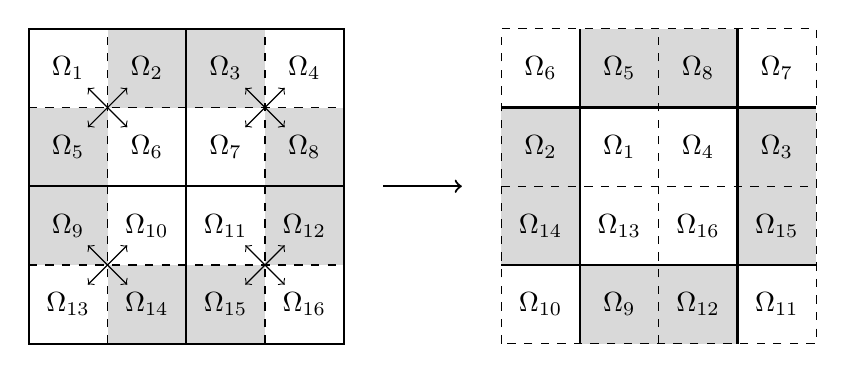
\begin{tikzpicture}
    % Original Grid

    \fill[gray!30] (1, 0) rectangle (3, 1);
    \fill[gray!30] (1, 3) rectangle (3, 4);

    \fill[gray!30] (0, 1) rectangle (1, 3);
    \fill[gray!30] (3, 1) rectangle (4, 3);

    \draw[thick] (0,0) rectangle (2,2);
    \draw[thick] (0,2) rectangle (2,4);
    \draw[thick] (2,0) rectangle (4,2);
    \draw[thick] (2,2) rectangle (4,4);
    \draw[dashed] (1,0) -- (1,4);
    \draw[dashed] (0,1) -- (4,1);
    \draw[dashed] (3,0) -- (3,4);
    \draw[dashed] (0,3) -- (4,3);

    \draw[<->] (0.75,0.75) -- (1.25,1.25);
    \draw[<->] (1.25,0.75) -- (0.75,1.25);

    \draw[<->] (2.75,0.75) -- (3.25,1.25);
    \draw[<->] (3.25,0.75) -- (2.75,1.25);

    \draw[<->] (0.75,2.75) -- (1.25,3.25);
    \draw[<->] (1.25,2.75) -- (0.75,3.25);

    \draw[<->] (2.75,2.75) -- (3.25,3.25);
    \draw[<->] (3.25,2.75) -- (2.75,3.25);

    \node at (0.5,3.5) {$\Omega_1$};
    \node at (1.5,3.5) {$\Omega_2$};
    \node at (0.5,2.5) {$\Omega_5$};
    \node at (1.5,2.5) {$\Omega_6$};

    \node at (2.5,3.5) {$\Omega_3$};
    \node at (3.5,3.5) {$\Omega_4$};
    \node at (2.5,2.5) {$\Omega_7$};
    \node at (3.5,2.5) {$\Omega_8$};

    \node at (0.5,1.5) {$\Omega_9$};
    \node at (1.5,1.5) {$\Omega_{10}$};
    \node at (0.5,0.5) {$\Omega_{13}$};
    \node at (1.5,0.5) {$\Omega_{14}$};

    \node at (2.5,1.5) {$\Omega_{11}$};
    \node at (3.5,1.5) {$\Omega_{12}$};
    \node at (2.5,0.5) {$\Omega_{15}$};
    \node at (3.5,0.5) {$\Omega_{16}$};

    % Arrow
    \draw[->, thick] (4.5,2) -- (5.5,2);

    % Transformed Grid
    \begin{scope}[shift={(6,0)}]
        \fill[gray!30] (1, 0) rectangle (3, 1);
        \fill[gray!30] (1, 3) rectangle (3, 4);

        \fill[gray!30] (0, 1) rectangle (1, 3);
        \fill[gray!30] (3, 1) rectangle (4, 3);

        \draw[dashed] (0,0) rectangle (4,4);

        \draw[dashed] (2,0) -- (2,4);
        \draw[dashed] (0,2) -- (4,2);

        \draw[thick] (1,0) -- (1,4);
        \draw[thick] (0,1) -- (4,1);
        \draw[thick] (3,0) -- (3,4);
        \draw[thick] (0,3) -- (4,3);

        \node at (0.5,3.5) {$\Omega_6$};
        \node at (1.5,3.5) {$\Omega_5$};
        \node at (0.5,2.5) {$\Omega_2$};
        \node at (1.5,2.5) {$\Omega_1$};

        \node at (2.5,3.5) {$\Omega_8$};
        \node at (3.5,3.5) {$\Omega_7$};
        \node at (2.5,2.5) {$\Omega_4$};
        \node at (3.5,2.5) {$\Omega_3$};

        \node at (0.5,1.5) {$\Omega_{14}$};
        \node at (1.5,1.5) {$\Omega_{13}$};
        \node at (0.5,0.5) {$\Omega_{10}$};
        \node at (1.5,0.5) {$\Omega_{9}$};

        \node at (2.5,1.5) {$\Omega_{16}$};
        \node at (3.5,1.5) {$\Omega_{15}$};
        \node at (2.5,0.5) {$\Omega_{12}$};
        \node at (3.5,0.5) {$\Omega_{11}$};
    \end{scope}
\end{tikzpicture}
\caption{Tobulo maišymo transformacija ant keturis kartus padidintų pradinių sąlygų}
\label{perfect-4x4-mix}
\end{figure}
\ref{perfect-4x4-mix}-ame pavyzdyje matome kaip atrodo tobulas išmaišymas praplėstų pradinių sąlygų atveju. Punktyrinės linijos žymi skirtingų medžiagų bendras sieneles t. y. tas sieneles, ties kuriomis aktyviai vyksta medžiagų reakcija. Paprastos linijos žymi sieneles, ties kuriomis susiduria tos pačios medžiagos sritys arba sieneles, kurios yra nukreiptos į išorę. Toks išmaišymas žymiai padidina reakcijos greitį todėl, kad visos sienelės tarp skirtingų medžiagų yra dar nesureagavusios ir turi didelį koncentracijų kontrastą.
\subsection{Modelio rezultatai didesnėse srityse}
Norint modeliuoti maišymą ir tirti šio proceso savybes skirtingo dydžio srityse turime atsižvelgti į tai, kad reakcijos modeliavimas skirtingo dydžio srityse be išmaišymo proceso gali suteikti nenuoseklius rezultatus, todėl pirmiausia turime išsiaiškinti esminius skirtumus tarp šių modelių. Viena svarbiausių modelio rezultatų savybių, kurias mes norėtume tirti yra reakcijos trukmė, todėl pažvelgsime kaip ji kinta priklausomai nuo srities dydžio kurią modeliuojame. Kaip aprašėme praeituose skyriuose, pradinę reakcijos sritį mes galime didinti keturis kartus ir tai daryti rekursyviai, todėl mūsų modeliuojamos sritys didės eksponentiškai.
\begin{figure}[h!]
    \centering
    \includegraphics[width=0.5\textwidth]{images/mixing/duration-order-T1000.png}

    \caption{Reakcijos trukmės priklausomybė nuo to, kiek kartų buvo padidintos pradinės sąlygos \eqref{fig:initial-condition-visual}. }

    \label{fig:duration-order-dependance}
\end{figure}
\subsection{Atsitiktinis maišymas didesnėse srityse}
\ref{fig:random-mix-larger-example}-ame pavyzdyje matome kaip atrodo atsitiktinis išmaišymas skaitiniame sprendinyje. Svarbu atkreipti dėmesį į tai, kad sumaišius sritis niekada neatsiras sričių, kuriose skirtingų medžiagų koncentracijos žymiai persidengia, taip yra todėl, kad vykstant maišymui visos tam tikroje srityje esančios medžiagos bus transformuotos tokiu pat būdu, o kadangi pradinėse sąlygose medžiagos nepersidengia -- išmaišytos medžiagos taip pat nepersidengs. Idealus rezultatas, kurio galime tikėtis atlikus atsitiktinį maišymą yra alternuojantis sričių išsidėstymas pagal koncentraciją kaip šachmatų lentoje -- tokiu būdu, difuzijos pagalba, skirtingas medžiagas laikančios sritys viena kitą galės pasiekti greičiausiai.

\newpage

\begin{figure}[h!]
  \centering
  \includegraphics[width=0.75\textwidth]{images/mixing/random-mix-ord-1-c1.png} \\ 
  \includegraphics[width=0.75\textwidth]{images/mixing/random-mix-ord-1-c2.png} \\
  \includegraphics[width=0.75\textwidth]{images/mixing/random-mix-ord-1-c3.png}
  \caption{Atsitiktinio maišymo poveikis skaitiniam sprendiniui. Modeliuojama sritis padidinta 4 kartus. Modelio parametrai atitinka reakciją vykstančia $1000\degree C$ temperatūroje. Modeliuojamos srities rezoliucija $80\times80$. Išmaišymo laikas -- $1\text{h}. $}
  \label{fig:random-mix-larger-example}
\end{figure}

Problema su kuria susidūrėme modeliuodami pačią mažiausią erdvės sritį išlieka ir čia -- erdvė per maža, kad išmaišymas sutrumpintų reakcijos laiką. Šiuo atveju nebūtų praktiška pateikti reakcijos trukmės nuo išmaišymo momento priklausomybės grafiką todėl, kad kiekvienam išmaišymo momentui reikėtų rasti kelis sprendinius. Vis dėl to galime pabandyti pasinaudoti pastebėjimu, kad optimalus išmaišymo laikas tobulo maišymo atveju yra apie 40min ir pabandyti ištirti kaip atsitiktinis maišymas paveikia reakcijos trukmę, kai maišymą atliekame šiuo, optimaliu momentu. 

\begin{figure}[h!]
  \centering
  \includegraphics[width=\textwidth]{images/mixing/sample-durations-random-mix.png}
  \caption{Vidutinės reakcijos trukmės skirtingo dydžio erdvėse, kai modeliuojamas atsitiktinis išmaišymas. Kiekvienam pavaizduotam srities dydžiui buvo padaryta 20 individualių sprendinių (bandymų) su atsitiktiniu išmaišymu. Išmaišymo laikas -- 40min. Pavaizduotas individualių sprendinių reakcijos trukmės laikas bei jų vidurkis.}
  \label{fig:random-samples}
\end{figure}

Pavyzdyje~\ref{fig:random-samples} matyti, kad erdvės didinimas daro neigiamą įtaką reakcijos trukmei: kuo didesnė modeliuojama erdvė, tuo ilgesnė vidutinė reakcijos trukmė. Manome, kad tokie rezultatai gaunami todėl, jog net ir padidinus erdvę 64 kartus, nesusidaro pakankamos sąlygos, leidžiančios atsitiktiniam maišymui paspartinti reakciją. Be to, veidrodiniu principu atkartotos pradinės sąlygos iš karto sukuria pakankamai palankų sričių išsidėstymą visoje reakcijos erdvėje, kurį atsitiktinis išmaišymas kaip tik suardo.

\subsection{Tobulo maišymo rezultatai didesnėse srityse}

\begin{figure}[h!]
  \centering
  \includegraphics[width=0.75\textwidth]{images/mixing/perfect-mix-ord-1-c1.png} \\ 
  \includegraphics[width=0.75\textwidth]{images/mixing/perfect-mix-ord-1-c2.png} \\
  \includegraphics[width=0.75\textwidth]{images/mixing/perfect-mix-ord-1-c3.png}
  \caption{Tobulo maišymo poveikis skaitiniam sprendiniui. Modeliuojama sritis padidinta 4 kartus. Modelio parametrai atitinka reakciją vykstančia $1000\degree C$ temperatūroje. Modeliuojamos srities rezoliucija $80\times80$. Išmaišymo laikas -- $1\text{h}. $}
  \label{fig:perfect-mix-larger-example}
\end{figure}

\begin{figure}[h!]
  \centering
  \includegraphics[width=0.75\textwidth]{images/mixing/duration-mix-moment-dependance-perfect.png}
  \caption{Reakcijos trukmės priklausomybė nuo išmaišymo momento, kai naudojamas tobulo maišymo modelis. Punktyrinės linijos žymi bazinę reakcijos trukmę skirtingo dydžio erdvėse, kai maišymas nevyksta. Legendoje matoma, kiek kartų didesnės erdvės buvo modeliuotos.}
  \label{fig:duration-mix-moment-perfect}
\end{figure}

Viena iš pageidautinų maišymo modelių savybių -- nuoseklus rezultatai, kurie būtų nepriklausomi nuo srities dydžio, kurią modeliuojame. Šiuo atveju pavyzdyje \ref{fig:duration-mix-moment-perfect} matome, kad priklausomybė šiek tiek svyruoja priklausomai nuo to, kiek kartų didesnėje srityje modeliuojame reakciją, tačiau optimalūs maišymo laikai beveik sutampa, o skirtumas tarp grafikų yra vertikalus. Taip pat galima pastebėti, kad didinant sritį grafikas konverguoją į \enquote{tikrąjį}. Šis rezultatas rodo, kad norint tiksliai išgauti optimalų maišymo laiką užtenka modeliuoti mažą erdvės sritį. 

Nors optimalūs maišymo laikai vizualiai beveik sutampa, gali būti naudinga ištirti, kaip jie kinta priklausomai nuo modeliuojamos srities dydžio su tikslesniu metodu. Tam galime pasinaudoti auksinio pjūvio paieškos algoritmu, kuris leidžia efektyviai rasti funkcijos minimumą tam tikrame intervale. Šis metodas paremtas tuo, kad kiekviename žingsnyje intervalas susiaurinamas remiantis auksinio pjūvio proporcija, sumažinant funkcijos kvietimų skaičių, kas šiuo atveju yra ypač svarbu iš praktinės pusės, nes norint apskaičiuoti reakcijos trukmę reikia modeliuoti visą reakciją, ką daryti užtrunka nemažai laiko (tolimesniems rezultatams išgauti prireikė kelių valandų paieškos). 

\begin{figure}[htbp]
  \centering
  \begin{subfigure}[t]{0.48\textwidth}
    \centering
    \includegraphics[width=\textwidth]{images/mixing/opt-mix-time.png}
    \caption{Optimalaus maišymo momento priklausomybė nuo to, kiek kartų padidinta sritis yra modeliuojama. }
    \label{fig:optimal-mix-time-order-dependance}
  \end{subfigure}
  \hfill
  \begin{subfigure}[t]{0.48\textwidth}
    \centering
    \includegraphics[width=\textwidth]{images/mixing/opt-duration.png}
    \caption{Optimalios reakcijos trukmės priklausomybė nuo to, kiek kartų padidinta sritis yra modeliuojama. }
    \label{fig:optimal-duration-order-dependance}
  \end{subfigure}
\end{figure}

\ref{fig:optimal-duration-order-dependance}-ame pavyzdyje matome, kad optimalus reakcijos laikas artėja prie \enquote{tikrosios} optimalios reikšmės, kai didiname srities dydį. Šis rezultatas nėra stebinantis, todėl, kad jau prieš tai matėme, kad tarp reakcijos trukmės nemaišant reagentų ir modeliuojamos srities dydžio egzistuoja labai panaši priklausomybė, kuri primena eksponentinį nykimą. Tiksliau pavaizdavus optimalaus maišymo momento priklausomybę nuo srities dydžio matome, kad optimalus maišymo momentas nėra toks nuoseklus kaip reakcijos trukmė ir neprimena eksponentinio nykimo, vis dėlto, skirtumas tarp šių momentų išlieka nedidelis -- apie 2min. 

\sectionnonum{Rezultatai ir išvados}

\subsection*{Rezultatai}

Šiame darbe buvo įgyvendinti šie uždaviniai:

\begin{itemize}
    \item Sudaryti kompiuteriniai YAG reakcijos modeliai remiantis išreikštiniu ir ADI skaitiniais metodais
    \item Teoriškai parodyta išreikštinio skaitinio modelio stabilumo sąlyga
    \item Sukurta kintamo laiko žingsnio strategija, kuri leidžia efektyviai modeliuoti YAG sintezės reakciją didelėse srityse naudojant ADI metodą
    \item Išreikštinio modelio rezultatai buvo verifikuojami ir buvo užtikrinta, kad modelis veikia korektiškai 
    \item Išmatuotas bei palygintas abiejų kompiuterinių modelių tikslumas ir efektyvumas
    \item Atsitiktinio ir tobulo maišymo modeliai integruoti į kompiuterinius (YAG) reakcijos modelius
    \item Ištirtas maišymo modelių poveikis įvairaus dydžio erdvėse ir nustatyta kaip skirtingų maišymo modelių savybės priklauso nuo erdvės dydžio
    \item Nustatyta reakcijos trukmės priklausomybė nuo maišymo momento, jos kaita didinant modeliuojamą erdvę. Paieškos algoritmu nustatyti optimalūs maišymo momentai.
\end{itemize}

\subsection*{Išvados}

Iš rezultatų analizės galima daryti šias išvadas:

\begin{itemize}
    
    \item Modeliuojant tobulą išmaišymą YAG reakcijoje, optimalus maišymo laikas išlieka reikšmingai nepakitęs, nepriklausomai nuo modeliuojamos srities dydžio todėl norint tiksliai apskaičiuoti optimalų maišymo laiką užtenka modeliuoti erdvės sritį, kuri yra vienos mikrodalelės dydžio

    \item Modeliuojant tobulą išmaišymą YAG reakcijoje, optimali reakcijos trukmė konverguoja didinant modeliuojamą sritį. Jei šis dydžio tikslumas yra svarbus -- daug kartų didinti modeliuojamą sritį nėra būtina

    \item Tobulo maišymo modelis atspindi savybes, kuriomis pasižymi realus maišymo procesas. Jei maišymas vyksta reakcijos pradžioje arba pabaigoje nepastebime jokio pokyčio reakcijos trukmėje, tačiau maišant kitais laiko momentais pastebime, kad reakcijos trukmė trumpėja. Šis maišymo modelis yra tinkamas modeliuoti išmaišymo procesą

    \item Kintamo laiko žingsnio strategija leidžia ypač efektyviai spręsti YAG reakcijos uždavinį, o įtaka sprendinio tikslumui yra nereikšminga

    \item Atsitiktinis maišymo modeliavimas neturi savybių, kuriomis turėtų pasižymėti bet koks maišymo modelis -- beveik visuomet reakcijos trukmė pailgėja. Tai galioja tada, kai modeliuojama erdvė yra dviejų dimensijų ir yra nedidelė palyginus su tikraja reakcijos erdve. Rezultatai rodo, kad net 64 kartus padidintoje srityje (originali sritis yra vienos mikrodalelės dydžio) vidutinis reakcijos laikas pailgėja daugiau nei 40 valandų, todėl laikome, kad atsitiktinis maišymo modelis yra nepraktiškas

\end{itemize}

\printbibliography[title = {Literatūra ir šaltiniai}]

\end{document}